\documentclass[11pt,a4paper]{article}
\usepackage[margin=2.4cm]{geometry}
\usepackage{amsmath,amssymb,mathtools,bm}
\usepackage{booktabs,array,xcolor,listings,enumitem}
\usepackage{tikz,pgfplots}
\usetikzlibrary{arrows.meta,positioning,calc,shapes.geometric}
\pgfplotsset{compat=1.16}
\usepackage[colorlinks=true,linkcolor=blue!50!black,urlcolor=blue!50!black]{hyperref}

\newcommand{\vv}{\mathbf v}
\newcommand{\nn}{\mathbf n}
\newcommand{\ff}{\mathbf f}
\newcommand{\Cm}{\mathsf C}
\newcommand{\dd}{\partial}
\newcommand{\fd}{\textsc{fdelmodc}}

\lstset{basicstyle=\ttfamily\footnotesize,breaklines=true,frame=single,
  backgroundcolor=\color{black!3},columns=fullflexible,keepspaces=true}

\title{Elastic wavefield reconstruction from boundary data in \fd\\[2pt]
\large Forward recording, equivalent (MPS) sources, time reversal and the backward kernel\\
--- all in \fd's sign convention}
\author{Implementation notes}
\date{Generated from the code state of 18 Sep 2026}

\begin{document}
\maketitle
\tableofcontents

%======================================================================
\section{Goal and summary}
%======================================================================
The goal is to implement the elastic wavefield-reconstruction scheme of
Aaker et al.\ (2020, \emph{GJI} \textbf{222}, 595--609) inside \fd. In a
\emph{forward} run the five fields $v_x,v_z,\tau_{xx},\tau_{zz},\tau_{xz}$ are
recorded on a closed rectangular contour $\Gamma=\partial\Omega$. In a second
run, with \emph{no real source}, equivalent sources built from the recorded
data are injected on the same contour, in reversed time order, and the wavefield
inside $\Omega$ is reconstructed.

Three things had to be right: (i) the injection must be the exact adjoint of
the extraction (same interpolation weights, same staggered positions);
(ii) the amplitudes of the equivalent sources must be consistent with the
discrete scaling of the \fd\ kernel; (iii) the \emph{signs} of the sources and
of the time-reversed data must be consistent with \fd's equations.

The sign point is the subtle one and is the main content of this note:

\begin{itemize}[leftmargin=1.2em]
\item With the ordinary (forward-time) kernel, a time-reversed recording can
  reconstruct \emph{either} the velocity \emph{or} the stress with its true sign,
  never both. The first implementation (default, \texttt{wfl\_bwd=0}) reconstructs
  velocity correctly and stress with flipped sign (measured amplitude ratio
  $k\approx-0.993$).
\item Running the same update code with $\Delta t\to-\Delta t$ (the
  \emph{backward kernel}, \texttt{wfl\_bwd=1}) makes the time-reversed fields
  \emph{native} solutions. All five fields then reconstruct with their true sign
  ($k\approx+0.993$ for all five, correlation $0.9997$).
\end{itemize}

Section~\ref{sec:results} gives the numbers and trace comparisons.

%======================================================================
\section{The \fd\ elastic scheme and its sign convention}
%======================================================================
\subsection{The update equations as coded}
The elastic kernel (\texttt{elastic4.c}, fourth order) updates, with $z$
increasing downward,
\begin{align*}
v_x &\mathrel{-}= \texttt{rox}\,\big[D_x\tau_{xx}+D_z\tau_{xz}\big], &
v_z &\mathrel{-}= \texttt{roz}\,\big[D_x\tau_{xz}+D_z\tau_{zz}\big],\\
\tau_{xx}&\mathrel{-}= \texttt{l2m}\,D_xv_x+\texttt{lam}\,D_zv_z, &
\tau_{zz}&\mathrel{-}= \texttt{l2m}\,D_zv_z+\texttt{lam}\,D_xv_x,\\
\tau_{xz}&\mathrel{-}= \texttt{mul}\,\big[D_zv_x+D_xv_z\big],
\end{align*}
where $D_x,D_z$ are the 4th-order staggered differences (coefficients $9/8$, $-1/24$)
\emph{without} the $1/\Delta x$ factor. That factor is built into the medium arrays
in \texttt{readModel.c} with \texttt{fac}$=\Delta t/\Delta x$:
\begin{equation}
\texttt{rox}=\frac{\Delta t}{\Delta x\,\rho_x},\quad
\texttt{roz}=\frac{\Delta t}{\Delta x\,\rho_z},\quad
\texttt{l2m}=\frac{\Delta t}{\Delta x}(\lambda+2\mu),\quad
\texttt{lam}=\frac{\Delta t}{\Delta x}\lambda,\quad
\texttt{mul}=\frac{\Delta t}{\Delta x}\mu .
\label{eq:coefs}
\end{equation}
Two facts used repeatedly below: (a) $\Delta t$ enters the kernel \emph{only}
through these five arrays; (b) the same $\Delta x$ (not a separate $\Delta z$) is
used on both axes.

\subsection{Continuous form and the stress sign}
Dividing by $\Delta t$ the coded update is the continuous system
\begin{equation}
\boxed{\;\rho\,\dd_t \vv+\nabla\!\cdot\bm\tau=\ff,\qquad
\dd_t\bm\tau+\Cm:\nabla\vv=\bm s\;}
\label{eq:fd}
\end{equation}
with, componentwise,
\[
\begin{aligned}
(\Cm:\nabla\vv)_{xx}&=(\lambda{+}2\mu)\dd_xv_x+\lambda\dd_zv_z,\quad
(\Cm:\nabla\vv)_{zz}=(\lambda{+}2\mu)\dd_zv_z+\lambda\dd_xv_x,\\
(\Cm:\nabla\vv)_{xz}&=\mu(\dd_zv_x+\dd_xv_z).
\end{aligned}
\]
Here $\ff$ (force density) and $\bm s$ (deformation-rate source) are the two
source terms. In the standard textbook form $\rho\dd_t\vv=\nabla\!\cdot\bm\sigma^{\rm std}$,
$\dd_t\bm\sigma^{\rm std}=\Cm:\nabla\vv$ (tension positive). Comparing with
\eqref{eq:fd},
\begin{equation}
\boxed{\;\bm\tau_{\fd}=-\bm\sigma^{\rm std}\;}
\end{equation}
i.e.\ \fd's stress is compression-positive (in the acoustic scheme $\tau_{zz}=p$).
In the rest of this document I write $\bm\tau$ (or $\tau_{xx},\tau_{zz},\tau_{xz}$)
for the \fd\ stress fields and use the code's names \texttt{txx,tzz,txz}.

\subsection{Comparison with the paper's convention}
Aaker et al.\ use the Aki--Richards form $\rho\dd_t\vv-\nabla\!\cdot\bm\tau^{\rm AR}=\ff$,
$\dd_t\bm\tau^{\rm AR}-\Cm:\nabla\vv=-\Cm:\bm h$, with $\bm\tau^{\rm AR}=\bm\sigma^{\rm std}=-\bm\tau_\fd$.
Substituting, the paper's system becomes exactly \eqref{eq:fd} with
$\ff=\ff^{\rm paper}$ and $\bm s=+\Cm:\bm h$. Their modified source functions are
\begin{equation}
\ff^{\rm paper}=\rho\oint_\Gamma\delta(\bm x-\bm x_r)\,\frac{\bm\tau^{\rm AR}\!\cdot\nn}{\rho(\bm x_r)}\,d\bm x_r\ \ (\text{eq.\,23}),\qquad
\bm h=-\oint_\Gamma\delta(\bm x-\bm x_r)\,\vv\otimes\nn\,d\bm x_r\ \ (\text{eq.\,24}),
\end{equation}
which in \fd\ variables read (using $\bm\tau^{\rm AR}=-\bm\tau_\fd$ and $\rho/\rho(\bm x_r)\approx1$)
\begin{equation}
\ff=-\bm\tau\!\cdot\nn\;\delta_\Gamma,\qquad
\bm s=-\Cm:(\vv\otimes\nn)\;\delta_\Gamma .
\label{eq:srcfd}
\end{equation}
I do not rely on the paper's signs, though: the next section derives
\eqref{eq:srcfd} directly from \eqref{eq:fd}, and the two agree.

%======================================================================
\section{Equivalent sources on a closed boundary}
%======================================================================
Let $\chi$ be the indicator of $\Omega$ ($\chi=1$ inside, $0$ outside) and
$\nn$ the \emph{outward} unit normal, so that $\nabla\chi=-\nn\,\delta_\Gamma$.
Let $(\vv,\bm\tau)$ be a solution of \eqref{eq:fd} with a true source
\emph{outside} $\Omega$ (or none). The truncated field $(\chi\vv,\chi\bm\tau)$ obeys
\begin{align}
\rho\dd_t(\chi\vv)+\nabla\!\cdot(\chi\bm\tau)&=\chi(\rho\dd_t\vv+\nabla\!\cdot\bm\tau)+\bm\tau\!\cdot\nabla\chi
=-\bm\tau\!\cdot\nn\,\delta_\Gamma,\\
\dd_t(\chi\bm\tau)+\Cm:\nabla(\chi\vv)&=\Cm:(\vv\otimes\nabla\chi)
=-\Cm:(\vv\otimes\nn)\,\delta_\Gamma .
\end{align}
So a wavefield that equals the true one inside $\Omega$ and is zero outside is
generated \emph{exactly} by the sources \eqref{eq:srcfd}, using no medium
knowledge except at $\Gamma$. This is the Huygens/representation-theorem
statement behind Aaker et al.\ (2020). In components, with the recorded
traction $\bm T=\bm\tau\!\cdot\nn$,
\begin{align}
T_x&=\tau_{xx}n_x+\tau_{xz}n_z, & T_z&=\tau_{xz}n_x+\tau_{zz}n_z,\\
\Cm:(\vv\otimes\nn)_{xx}&=(\lambda{+}2\mu)v_xn_x+\lambda v_zn_z, &
\Cm:(\vv\otimes\nn)_{zz}&=\lambda v_xn_x+(\lambda{+}2\mu)v_zn_z,\\
\Cm:(\vv\otimes\nn)_{xz}&=\mu\,(v_xn_z+v_zn_x). &&
\end{align}
So the recorded $\tau$ feeds the \emph{force} on $v_x,v_z$, and the recorded $\vv$
feeds the \emph{deformation-rate} sources on $\tau_{xx},\tau_{zz},\tau_{xz}$.
That is the ``MPS'' (modified physical sources) structure.

\begin{figure}[h]
\centering
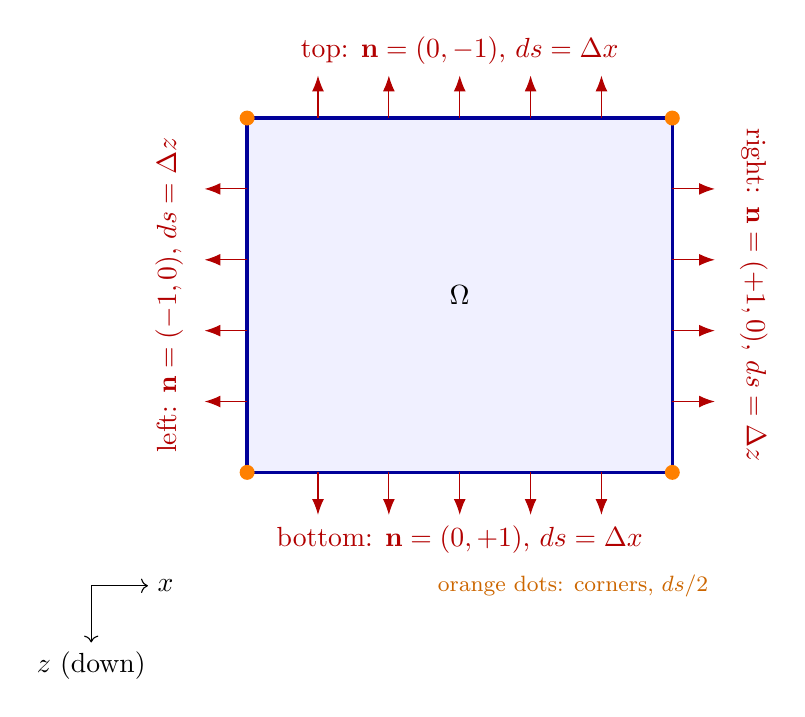
\begin{tikzpicture}[scale=0.9]
 \fill[blue!6] (0,0) rectangle (6,5);
 \draw[very thick,blue!60!black] (0,0) rectangle (6,5);
 \node at (3,2.5) {$\Omega$};
 \foreach \x in {1,2,...,5}{
   \draw[-{Latex[length=2mm]},red!70!black] (\x,5) -- (\x,5.6);
   \draw[-{Latex[length=2mm]},red!70!black] (\x,0) -- (\x,-0.6);}
 \foreach \y in {1,2,...,4}{
   \draw[-{Latex[length=2mm]},red!70!black] (0,\y) -- (-0.6,\y);
   \draw[-{Latex[length=2mm]},red!70!black] (6,\y) -- (6.6,\y);}
 \foreach \c in {(0,0),(6,0),(0,5),(6,5)} \fill[orange] \c circle (3pt);
 \node[red!70!black] at (3,5.95) {top: $\nn=(0,-1)$, $ds=\Delta x$};
 \node[red!70!black] at (3,-0.95) {bottom: $\nn=(0,+1)$, $ds=\Delta x$};
 \node[red!70!black,rotate=90] at (-1.1,2.5) {left: $\nn=(-1,0)$, $ds=\Delta z$};
 \node[red!70!black,rotate=-90] at (7.15,2.5) {right: $\nn=(+1,0)$, $ds=\Delta z$};
 \node[orange!80!black,font=\footnotesize] at (4.6,-1.6) {orange dots: corners, $ds/2$};
 \draw[->] (-2.2,-1.6)--(-1.4,-1.6) node[right]{$x$};
 \draw[->] (-2.2,-1.6)--(-2.2,-2.4) node[below]{$z$ (down)};
\end{tikzpicture}
\caption{Contour $\Gamma$ of $\Omega=[x_1,x_2]\times[z_1,z_2]$. Red arrows: outward normals.
Orange dots: the four corners, which carry half weight.}
\label{fig:geom}
\end{figure}

%======================================================================
\section{Discretisation on the staggered grid}
%======================================================================
\subsection{Contour points, normals, corners}
\texttt{defineRecBoundary.c} builds the contour with spacing $\Delta x$ on the top
and bottom faces and $\Delta z$ on the left and right faces. The top and bottom
faces include the four corners; the left and right faces exclude them (so no
duplicate points). For $\Omega=[500,2500]^2$~m at $4$~m this gives
$2\cdot501+2\cdot499=2000$ contour points. Each point stores its position, its
outward normal (Fig.~\ref{fig:geom}) and an \texttt{is\_corner} flag.

\paragraph{Corner weighting.}
At the four Cartesian corners the normal is discontinuous. Aaker et al.\ (Sec.~5.1)
identify this as the largest error source and fix it with weight $1/2$ on the
corner points; the code does this by halving $ds$ there.

\subsection{One interpolation table per field}
The five fields live at different staggered positions. From \texttt{readModel.c}
(with the boundary padding indices \texttt{ioXx, ioZz, \dots}) the physical
position of field element \texttt{f[ix*naz+iz]} is
\begin{center}
\begin{tabular}{lll}\toprule
field & $x$ offset & $z$ offset\\\midrule
\texttt{vx}  & $(\tfrac12-\texttt{ioXx})\Delta x$ & $-\texttt{ioXz}\,\Delta z$\\
\texttt{vz}  & $-\texttt{ioZx}\,\Delta x$ & $(\tfrac12-\texttt{ioZz})\Delta z$\\
\texttt{txx,tzz} & $-\texttt{ioPx}\,\Delta x$ & $-\texttt{ioPz}\,\Delta z$\\
\texttt{txz} & $(\tfrac12-\texttt{ioTx})\Delta x$ & $(\tfrac12-\texttt{ioTz})\Delta z$\\\bottomrule
\end{tabular}
\end{center}
(index $\times$ spacing $+$ offset; the padding terms encode the absorbing-layer
shift). For each field, \texttt{bndinterpInit} (file \texttt{bndinterp.c}) computes
for every contour point the base index and four bilinear weights
$w_{00},w_{01},w_{10},w_{11}$ and a \texttt{valid} flag for the $2\times2$ footprint.

The single primitive \texttt{bndinterp(inject, \dots)} uses those weights in two
directions:
\begin{itemize}[leftmargin=1.2em]
\item \texttt{inject=0} (extract): $d_i=\sum w\,\texttt{field}[\dots]$;
\item \texttt{inject=1} (inject): $\texttt{field}[\dots]\mathrel{+}=w\,d_i$
  (it never zeroes the live field).
\end{itemize}
Because both directions use the \emph{same} table, injection is the exact
adjoint of extraction by construction. This was checked by an adjoint (dot-product)
test of the primitive.

\subsection{Amplitude: the $ds/\Delta z$ factor}
The equivalent sources \eqref{eq:srcfd} are line densities on $\Gamma$; the
kernel wants a per-node increment. Take the force term. A discrete boundary
point represents $F\,ds$ (force per length times length), spread over the
cell area $\Delta x\Delta z$:
\[
\Delta v=\frac{\Delta t}{\rho}\,\frac{F\,ds}{\Delta x\,\Delta z}
=\underbrace{\frac{\Delta t}{\rho\,\Delta x}}_{\texttt{rox}}\,F\,\frac{ds}{\Delta z}.
\]
The same steps for the stress sources give $\Delta\tau=\texttt{l2m}\,(\dots)\,ds/\Delta z$
etc. So every increment is (medium array at the contour point)$\times ds/\Delta z\times$
(recorded data), and \emph{not} $\Delta x\,ds\times\dots$ (an earlier version had
this wrong: units of $\texttt{rox}\,\Delta x\,ds\,T$ are m$^3$/s, whereas
$\texttt{rox}\,(ds/\Delta z)\,T$ is m/s).
$\Delta z$ is the uniform normaliser because \texttt{fac}$=\Delta t/\Delta x$ is used for
both axes. With this scaling the reconstructed amplitude at the test point is
within about $0.7\%$ of the forward one (Sec.~\ref{sec:results}).
The medium values (\texttt{rox}, \texttt{roz}, \texttt{l2m}, \texttt{lam},
\texttt{mul}) are sampled at the contour point through the field's own table,
and $\rho(\bm x)/\rho(\bm x_r)$ is taken as 1.

%======================================================================
\section{The forward (recording) run}
%======================================================================
Command-line: \texttt{wfl\_recon=1 wfl\_x1 wfl\_x2 wfl\_z1 wfl\_z2 wfl\_file=\dots}.
The run is an ordinary \fd\ elastic run with the real source (in the demo a
vertical force, \texttt{src\_type=1 src\_orient=1}, Ricker $f_p=15$~Hz at
$(1500,1500)$). At the end of \emph{every} time step $it$, in the OpenMP-master
block of the main loop, after \texttt{elastic4()} has updated velocities and
stresses, \texttt{storeBoundaryWav} does
\begin{lstlisting}
bndinterp(0,0, vx , naz, tmp, rb.vx ) ; bs_vx [i*nt+it] = tmp[i];   /* likewise vz,txx,tzz,txz */
\end{lstlisting}
and the arrays \texttt{bs\_*} (size $n_{\rm contour}\times n_t$, full resolution,
not decimated by \texttt{dtrcv}) are written by \texttt{writeBoundaryWav} to
\texttt{wfl\_file}. The recorded values are the raw \fd\ fields, i.e.\ the
compression-positive $\bm\tau_\fd$ and the true $\vv$. Nothing is negated at
recording.

Timing note: the store is after the full step, so all five recorded fields are
taken at the same loop index although $\vv$ and $\bm\tau$ are staggered in time by
a half step. This half-step mismatch is one plausible source of the 1--2 sample
lags reported in Sec.~\ref{sec:results}; it has not been isolated by a dedicated test.

\begin{figure}[h]
\centering
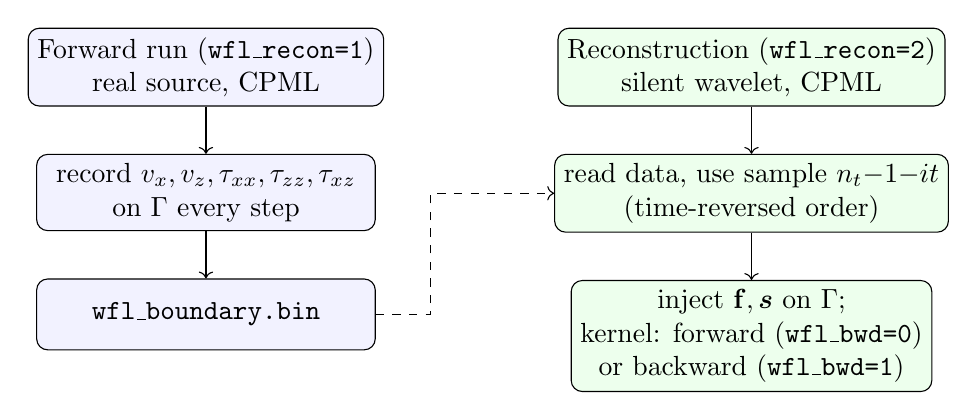
\begin{tikzpicture}[node distance=6mm,
  box/.style={draw,rounded corners,align=center,minimum width=4.3cm,minimum height=9mm,fill=blue!5},
  bx2/.style={draw,rounded corners,align=center,minimum width=4.3cm,minimum height=9mm,fill=green!7}]
 \node[box] (a) {Forward run (\texttt{wfl\_recon=1})\\ real source, CPML};
 \node[box,below=of a] (b) {record $v_x,v_z,\tau_{xx},\tau_{zz},\tau_{xz}$\\ on $\Gamma$ every step};
 \node[box,below=of b] (c) {\texttt{wfl\_boundary.bin}};
 \node[bx2,right=2.2cm of a] (d) {Reconstruction (\texttt{wfl\_recon=2})\\ silent wavelet, CPML};
 \node[bx2,below=of d] (e) {read data, use sample $n_t{-}1{-}it$\\ (time-reversed order)};
 \node[bx2,below=of e] (f) {inject $\ff,\bm s$ on $\Gamma$;\\ kernel: forward ($\texttt{wfl\_bwd=0}$)\\ or backward ($\texttt{wfl\_bwd=1}$)};
 \draw[->] (a)--(b); \draw[->] (b)--(c); \draw[->,dashed] (c.east) -- ++(0.7,0) |- (e.west);
 \draw[->] (d)--(e); \draw[->] (e)--(f);
\end{tikzpicture}
\caption{The two runs.}
\end{figure}

%======================================================================
\section{Reconstruction run: time reversal}
%======================================================================
\subsection{Setup common to both modes}
The reconstruction run has \emph{no} real source. \fd's command line has no ``no
source'' mode (a \texttt{NULL} source file crashes \texttt{defineSource.c}), so
the script passes a wavelet multiplied by exactly $0$ (\texttt{sugain scale=0.0};
note \texttt{makewave scale=0} means ``do not scale'', not ``zero''). The script
verifies at runtime that this wavelet is exactly zero, and \texttt{applySource.c}
skips zero-amplitude sources, so the run is driven \emph{only} by the boundary
injection.

At loop step $it$ (loop time $s=it\,\Delta t$) the sample used is $n_t-1-it$, i.e.\ the
recording is played backwards. In terms of the forward solution $(\vv,\bm\tau)(t)$ with
$T=t_{\rm mod}$ define the time-reversed fields
\begin{equation}
\tilde\vv(s)=\vv(T-s),\qquad \tilde{\bm\tau}(s)=\bm\tau(T-s).
\end{equation}
These are exactly what is read from the file at loop time $s$.

\subsection{What time reversal does to the equations}
Since $\dd_s\tilde\vv=-(\dd_t\vv)(T-s)$ and likewise for $\tilde{\bm\tau}$,
\eqref{eq:fd} (source-free) gives
\begin{equation}
\rho\,\dd_s\tilde\vv=+\nabla\!\cdot\tilde{\bm\tau},\qquad
\dd_s\tilde{\bm\tau}=+\Cm:\nabla\tilde\vv .
\label{eq:rev}
\end{equation}
Both right-hand sides have the \emph{opposite} sign to the forward system
\eqref{eq:fd}, which is the reason the forward kernel cannot reproduce
$(\tilde\vv,\tilde{\bm\tau})$ directly. Two other sign choices \emph{do} solve
the forward system:
\begin{align}
\text{Option S:}&\quad(\tilde\vv,\,-\tilde{\bm\tau}),\\
\text{Option V:}&\quad(-\tilde\vv,\,+\tilde{\bm\tau}).
\end{align}
(Check Option S: $\rho\dd_s\tilde\vv=\nabla\!\cdot\tilde{\bm\tau}=-\nabla\!\cdot(-\tilde{\bm\tau})$ and
$\dd_s(-\tilde{\bm\tau})=-\Cm:\nabla\tilde\vv$, both of the form \eqref{eq:fd}.) Exactly one of $\vv,\bm\tau$ must
therefore be negated with the forward kernel.

\subsection{Default mode (\texttt{wfl\_bwd=0}): forward kernel, Option S}
This is the first implementation and is unchanged by the backward-kernel work.
The truncation formulas \eqref{eq:srcfd} applied to the Option-S field
$(\vv_c,\bm\tau_c)=(\tilde\vv,-\tilde{\bm\tau})$ give
\begin{equation}
\ff=+\tilde{\bm\tau}\!\cdot\nn\,\delta_\Gamma,\qquad
\bm s=-\Cm:(\tilde\vv\otimes\nn)\,\delta_\Gamma .
\end{equation}
In the code, at load time \texttt{bs\_vx, bs\_vz} are multiplied by $-1$
(so the loaded $v$ is $-\tilde v$) and \texttt{injectBoundary} then adds, with $ds$
as above and the (positive) medium arrays,
\begin{lstlisting}
tx = txx*nx + txz*nz;   tz = txz*nx + tzz*nz;           /* traction, raw tau  */
d_vx  = rox*(ds/dz)*tx;              d_vz  = roz*(ds/dz)*tz;
d_txx = (ds/dz)*(l2m*vxr*nx + lam*vzr*nz);              /* vxr = -vtilde     */
d_tzz = (ds/dz)*(lam*vxr*nx + l2m*vzr*nz);
d_txz = (ds/dz)*mul*(vxr*nz + vzr*nx);
\end{lstlisting}
which is $\ff=+\tilde{\bm\tau}\!\cdot\nn$ and $\bm s=-\Cm:(\tilde\vv\otimes\nn)$ as required. The field this run
produces is therefore $(\tilde\vv,-\tilde{\bm\tau})$: the velocity has the true
sign and \textbf{the stress is flipped}. This matches the measurement
($k_{v}\approx+0.993$, $k_\tau\approx-0.993$) and is not a bug in the source
amplitude or in the interpolation: it is the sign that the forward kernel
\emph{must} produce for this choice (Option S). Choosing instead Option V would
flip the velocity and leave the stress correct.

\subsection{Backward kernel (\texttt{wfl\_bwd=1})}
\paragraph{Idea.}
Because $\Delta t$ enters the kernel only through
\texttt{rox, roz, l2m, lam, mul} \eqref{eq:coefs}, negating those five arrays
runs the very same update code with $\Delta t\to-\Delta t$:
\[
\tilde v \mathrel{+}= |\texttt{rox}|\,D\tilde\tau,\quad
\tilde\tau \mathrel{+}= |\texttt{l2m}|\,D\tilde v+\dots
\]
i.e.\ the discretisation of $\rho\dd_s\tilde\vv=+\nabla\!\cdot\tilde{\bm\tau}$,
$\dd_s\tilde{\bm\tau}=+\Cm:\nabla\tilde\vv$, which is precisely the time-reversed
system \eqref{eq:rev}. So $(\tilde\vv,\tilde{\bm\tau})$, both with their true
signs, are \emph{native} solutions and no field has to be negated.
(Leapfrog is symmetric in $\Delta t$, so this is stable under the same CFL condition
in the lossless interior.)

\paragraph{Sources.}
In the loop time $s$ the equations with sources are
$\rho\dd_s\tilde\vv-\nabla\!\cdot\tilde{\bm\tau}=\ff_b$,
$\dd_s\tilde{\bm\tau}-\Cm:\nabla\tilde\vv=\bm s_b$. Truncating with $\chi$ as in
Sec.~3, and using $\nabla\chi=-\nn\delta_\Gamma$,
\begin{align}
\rho\dd_s(\chi\tilde\vv)-\nabla\!\cdot(\chi\tilde{\bm\tau})&=-\tilde{\bm\tau}\!\cdot\nabla\chi=+\tilde{\bm\tau}\!\cdot\nn\,\delta_\Gamma,\\
\dd_s(\chi\tilde{\bm\tau})-\Cm:\nabla(\chi\tilde\vv)&=-\Cm:(\tilde\vv\otimes\nabla\chi)=+\Cm:(\tilde\vv\otimes\nn)\,\delta_\Gamma .
\end{align}
So in the backward kernel
\begin{equation}
\boxed{\ \ff_b=+\tilde{\bm\tau}\!\cdot\nn\,\delta_\Gamma,\qquad
\bm s_b=+\Cm:(\tilde\vv\otimes\nn)\,\delta_\Gamma\ }
\end{equation}
with \emph{unnegated} reversed data. Each increment is added with time step
$+\Delta t$ in loop time, so the coefficients that multiply $ds/\Delta z$ are the
\emph{positive} magnitudes $|\texttt{rox}|$, etc. \texttt{injectBoundaryBwd.c} is a
copy of \texttt{injectBoundary.c} that samples the (now negated) arrays through the
same tables and multiplies by $-1$ to recover the positive values (not
\texttt{fabsf}, since $\lambda$ can be negative in general). The formulas are
otherwise the ones of the listing above, with \texttt{vxr}$=+\tilde v_x$.

\paragraph{Consistency check with the default mode.}
Relative to the default mode the backward kernel flips the sign of the coupling
(negated arrays) \emph{and} of the injected velocity sources, which is what turns
Option S into the native solution. The 1D analogue of this scheme was verified
independently in a pure-python test: stress $k=+1.00$, velocity $k=+1.00$, leakage $\approx0.03$.

\paragraph{What the switch changes in the code.}
With \texttt{wfl\_bwd=1} (only allowed together with \texttt{wfl\_recon=2}),
\texttt{fdelmodc.c} does three things, all behind \texttt{if (mod.wfl\_bwd)}:
\begin{enumerate}[leftmargin=1.4em]
\item after \texttt{readModel}, negate \texttt{rox, roz, l2m, lam, mul} (whole arrays);
\item skip the negation of \texttt{bs\_vx, bs\_vz} at load;
\item call \texttt{injectBoundaryBwd} instead of \texttt{injectBoundary}.
\end{enumerate}
With the flag unset (default) every code path is byte-for-byte the original one.

\paragraph{CPML.}
The CPML coefficients $b,c,i_k$ are computed from
\texttt{mod.dt, cp\_min, dx, npml} and do not depend on the model arrays. In the
PML cells the update is $\psi=b\psi+c\,d;\ d\leftarrow i_kd+\psi;\ \tau\mathrel{-}=\texttt{l2m}(\dots)$,
so negating \texttt{l2m} flips the coupling consistently while the memory
recursion remains a decaying filter in loop time. In the test this worked (no
instability, $k\approx+0.993$), but the CPML in reversed time is not proven
stable in general; it has only been observed to behave.

%======================================================================
\section{Where things are in the code}
%======================================================================
\begin{center}\small
\begin{tabular}{p{4.1cm}p{10.3cm}}\toprule
file & role\\\midrule
\texttt{fdelmodc.h} & \texttt{modPar}: \texttt{wfl\_recon, wfl\_x1..wfl\_z2, wfl\_file}, \texttt{wfl\_bwd}; include guard added\\
\texttt{getParameters.c} & parses the \texttt{wfl\_*} parameters; \texttt{wfl\_bwd} defaults to 0, error unless \texttt{wfl\_recon=2}; elastic scheme only\\
\texttt{bndinterp.c/.h} & bilinear weight tables; extract/inject primitive (adjoint pair)\\
\texttt{bndsrc.h} & \texttt{bndSrcPar} struct, prototypes, derivation comments\\
\texttt{defineRecBoundary.c} & contour, normals, corner flags, five staggered tables\\
\texttt{storeBoundaryWav.c} & extraction each step (forward run)\\
\texttt{writeBoundaryWav.c}, \texttt{readBoundaryWav.c} & raw binary I/O with consistency checks\\
\texttt{injectBoundary.c} & default injection (forward kernel, Option S)\\
\texttt{injectBoundaryBwd.c} & backward-kernel injection, un-negated coefficients\\
\texttt{fdelmodc.c} & allocation, load, main-loop store/inject calls, the three \texttt{wfl\_bwd} switches\\
\texttt{Makefile} & new sources; header-dependency line (stale objects caused a struct-layout crash once)\\
\texttt{demo/wfl\_recon.scr} & forward run + default reconstruction + checks\\
\texttt{demo/wfl\_recon\_bwd.scr} & backward-kernel reconstruction, new output names\\
\texttt{backward\_kernel\_backup/} & original files, patch, \texttt{CHANGES.md} with revert commands\\\bottomrule
\end{tabular}
\end{center}

\paragraph{Main-loop sequence at step $it$.}
\texttt{elastic4()} (velocities, then stresses, CPML) $\rightarrow$ in the master
block either \texttt{storeBoundaryWav(it)} (mode 1) or
\texttt{injectBoundary[Bwd](\dots, nt-1-it, \dots)} (mode 2) $\rightarrow$ receiver
and snapshot output. The injection therefore happens after the step's update, so
a velocity source is seen by the stress update only in the next step (a
half-step timing approximation relative to injecting at each field's natural
half step).

\paragraph{Demo parameters.}
$\Delta x=\Delta z=4$~m, model $3100\times3100$~m, homogeneous
$c_p=2300$, $c_s=1300$~m/s, $\rho=2000$~kg/m$^3$; $\Delta t=0.5$~ms,
Ricker $f_p=15$~Hz, $t_0=0.15$~s; $\Omega=[500,2500]^2$~m; source at
$(1500,1500)$; independent receiver at $(2200,800)$; \texttt{tmod}$=1.1$~s
(snapshots from 0.1 to 1.1 s each 0.05 s, so frame $k$ of the reconstruction mirrors frame
$N{-}1{-}k$ of the forward run); CPML with 20 cells on all four sides
(\texttt{left=right=top=bottom=2}).

%======================================================================
\section{Results}\label{sec:results}
%======================================================================
The independent receiver at $(2200,800)$ records the forward field (from the forward
run) and the reconstructed field (from the reconstruction run, whose loop time
runs backwards). For the comparison the reconstructed trace is reversed in
time. Amplitude ratio $k$ is the least-squares factor in
$\text{recon}\approx k\cdot\text{forward}$, at the best integer-sample lag within $\pm6$ samples.

\begin{center}
\begin{tabular}{lrrrrrr}\toprule
 & \multicolumn{3}{c}{default (\texttt{wfl\_bwd=0})} & \multicolumn{3}{c}{backward kernel (\texttt{wfl\_bwd=1})}\\
 \cmidrule(lr){2-4}\cmidrule(lr){5-7}
field & lag & corr & $k$ & lag & corr & $k$\\\midrule
\texttt{vx}  & 2 & $+0.9997$ & $+0.9926$ & 2 & $+0.9997$ & $+0.9926$\\
\texttt{vz}  & 2 & $+0.9997$ & $+0.9925$ & 2 & $+0.9997$ & $+0.9925$\\
\texttt{txx} & 1 & $-0.9997$ & $-0.9927$ & 1 & $+0.9997$ & $+0.9927$\\
\texttt{tzz} & 1 & $-0.9997$ & $-0.9926$ & 1 & $+0.9997$ & $+0.9926$\\
\texttt{txz} & 1 & $-0.9997$ & $-0.9923$ & 1 & $+0.9997$ & $+0.9923$\\\bottomrule
\end{tabular}
\end{center}

The default run reproduces the velocity and returns the stress with the wrong
sign; the backward kernel returns all five with $k\approx+0.993$. The lag is one
to two samples ($0.5$--$1$~ms at $\Delta t=0.5$~ms). The amplitude is about $0.7\%$
low in both modes; its cause (bilinear smoothing, the $ds/\Delta z$ point-source
normalisation, or the small timing offset) has not been isolated.

Figure~\ref{fig:traces} overlays the forward trace and the time-reversed
reconstruction (amplitudes normalised to the forward maximum), around the
P-wave arrival, for $v_z$ and $\tau_{xz}$.

\begin{figure}[h]
\centering
\pgfplotsset{tr/.style={width=0.48\textwidth,height=4.6cm,xmin=0.50,xmax=0.70,
  xlabel={time (s)},tick label style={font=\footnotesize},label style={font=\footnotesize},
  title style={font=\footnotesize},legend style={font=\tiny,draw=none,fill=none},grid=both,
  grid style={black!8}}}
\begin{tikzpicture}
\begin{axis}[tr,title={default mode: $v_z$},legend pos=north east]
 \addplot[black,thick] table[x=t,y=f] {tr_vz.dat};
 \addplot[red,dashed,thick] table[x=t,y=orig] {tr_vz.dat};
 \legend{forward,reconstr.}
\end{axis}
\begin{axis}[tr,at={(0.52\textwidth,0)},title={default mode: $\tau_{xz}$ (flipped)},legend pos=north east]
 \addplot[black,thick] table[x=t,y=f] {tr_txz.dat};
 \addplot[red,dashed,thick] table[x=t,y=orig] {tr_txz.dat};
\end{axis}
\end{tikzpicture}\\[3mm]
\begin{tikzpicture}
\begin{axis}[tr,title={backward kernel: $v_z$}]
 \addplot[black,thick] table[x=t,y=f] {tr_vz.dat};
 \addplot[blue!70!black,dashed,thick] table[x=t,y=bwd] {tr_vz.dat};
\end{axis}
\begin{axis}[tr,at={(0.52\textwidth,0)},title={backward kernel: $\tau_{xz}$}]
 \addplot[black,thick] table[x=t,y=f] {tr_txz.dat};
 \addplot[blue!70!black,dashed,thick] table[x=t,y=bwd] {tr_txz.dat};
\end{axis}
\end{tikzpicture}
\caption{Point $(2200,800)$: forward trace (black) and time-reversed reconstruction (dashed).
Top: default mode, the stress is inverted. Bottom: backward kernel, both have the true sign.}
\label{fig:traces}
\end{figure}

\paragraph{Snapshots.}
\texttt{wfl\_recon\_bwd.scr} reverses the frame order of the reconstruction cube and
forms \texttt{suop2 op=diff} against the forward cube for all five fields with
\emph{no} sign flips; inside $\Omega$ the difference should be small. Outside
$\Omega$ the reconstruction is ideally zero, so the difference there just equals the forward field.
I have not quantified the snapshot differences numerically in this document; the
trace table above is the quantitative evidence.

%======================================================================
\section{Known limitations and open items}
%======================================================================
\begin{enumerate}[leftmargin=1.4em]
\item \textbf{Source inside $\Omega$.} The demo source sits inside $\Omega$.
  Aaker et al.\ (Sec.~3.4) note that boundary injection then reproduces the
  wavefield plus a spurious ``homogeneous Green's function'' part
  (after the wave has focused at the source position and expanded again), to be
  removed by also injecting the negated original source. That correction is
  \emph{not} implemented. The compared window ($\approx0.5$--$0.7$~s forward time)
  corresponds to loop times before the focus at the source ($\approx T-t_0\approx0.95$~s),
  and by an arrival-time estimate the ghost cannot reach the test point within the
  run, so the comparison at that point is expected to be unaffected; this is an
  estimate, not a test.
\item \textbf{Initial condition.} The construction assumes the forward field inside
  $\Omega$ has vanished by $t_{\rm mod}$. With $t_{\rm mod}=1.1$~s the S-wave has
  not yet fully left $\Omega$ (S-travel time to the far corners is about
  $1.24$~s), so the reconstruction start state is slightly incomplete. The effect
  has not been quantified.
\item \textbf{Half-step staggering.} Storage and injection happen after the full
  step, not at each field's own half step, giving the observed 1--2 sample lag
  (explanation plausible, not proven).
\item \textbf{Absorbing layers.} The former taper (\texttt{ntaper}, type 4) damps only the
  velocities and is not adequate; CPML (type 2) is used. CPML in reversed time
  works in the test but has no stability proof.
\item \textbf{Scope.} Elastic scheme only, homogeneous test, rectangular $\Omega$,
  \texttt{iorder=4} exercised. Heterogeneity, other orders and viscoelastic media
  are untested.
\end{enumerate}

%======================================================================
\section{Reproducing and reverting}
%======================================================================
\begin{lstlisting}
cd fdelmodc && make                     # builds ../fdelmodc
cd demo
./wfl_recon.scr                         # forward run + default reconstruction (Option S)
./wfl_recon_bwd.scr                     # backward-kernel reconstruction (needs the first run)
\end{lstlisting}
\begin{sloppypar}
Revert the backward-kernel work completely by restoring the five files from
the folder \texttt{backward\_kernel\_backup/original/}, deleting
\texttt{injectBoundaryBwd.c} and rebuilding (details in
\texttt{backward\_kernel\_backup/CHANGES.md}); or simply do not pass
\texttt{wfl\_bwd=1}.
\end{sloppypar}

\end{document}
